% !TeX spellcheck = sk_SK-Slovak
\documentclass[a4paper]{article}
\usepackage[slovak]{babel}
\usepackage[utf8]{inputenc}
\usepackage[T1]{fontenc}
\usepackage{a4wide}
\usepackage{amsmath}
\usepackage{amsfonts}
\usepackage{amssymb}
\usepackage{mathrsfs}
\usepackage[small,bf]{caption}
\usepackage{subcaption}
\usepackage{xcolor}
\usepackage{graphicx}
\usepackage{enumerate}
\usepackage{hyperref}
\usepackage{fancyvrb}
\usepackage{listings}
%\usepackage{lstautogobble}
\usepackage{stmaryrd}

\lstset{basicstyle=\ttfamily,
	mathescape=true,
	escapeinside=||%,
	%autogobble
}


\fvset{tabsize=4}


\pagestyle{empty}
\setlength{\parindent}{0pt}

\newenvironment{modenumerate}
{\enumerate\setupmodenumerate}
{\endenumerate}

\newif\ifmoditem
\newcommand{\setupmodenumerate}{%
	\global\moditemfalse
	\let\origmakelabel\makelabel
	\def\moditem##1{\global\moditemtrue\def\mesymbol{##1}\item}%
	\def\makelabel##1{%
		\origmakelabel{##1\ifmoditem\rlap{\mesymbol}\fi\enspace}%
		\global\moditemfalse}%
}

\makeatletter
\def\@seccntformat#1{%
	\expandafter\ifx\csname c@#1\endcsname\c@section\else
	\csname the#1\endcsname\quad
	\fi}
\makeatother

\begin{document} 
	
\pagenumbering{arabic}
\pagestyle{plain}

\begin{center}
	\sc\large
	Formálne metódy tvorby softvéru\\
	Domáca úloha 1 
\end{center}

Autor: Marián Kravec

\section{1.)}

Dokážeme sporom, uvažujme, že existuje $(P,Q) \in S \land (P,Q) \notin \sim$, z definície silnej bisimulácie až na $\sim$ vieme, že platí $(P',Q') \in \sim S \sim$, z toho by malo vyplývať $(P',Q') \in \sim$ a keďže $P'$ a $Q'$ vznikli z $P$ a $Q$ rovnakým procesom tak by malo platiť $(P,Q) \in \sim$ čo je spor s predpokladom a preto musí platiť $S \subseteq \sim$

\section{2.)}

\begin{enumerate}[a)]
	\item a.Nil a a.Nil + a.Nil  ->  Áno
	\item a.b.Nil + a.c.Nil a a.(b.Nil + c.Nil)  -> Nie
	\item a.Nil|b.Nil a a.b.Nil + b.a.Nil  -> Áno
	\item a.Nil|a.Nil a a.Nil  -> Nie
	\item a.Nil|a.Nil a a.a.Nil + a.a.Nil  -> Áno
\end{enumerate}

\begin{figure}[!h]
	\centering
	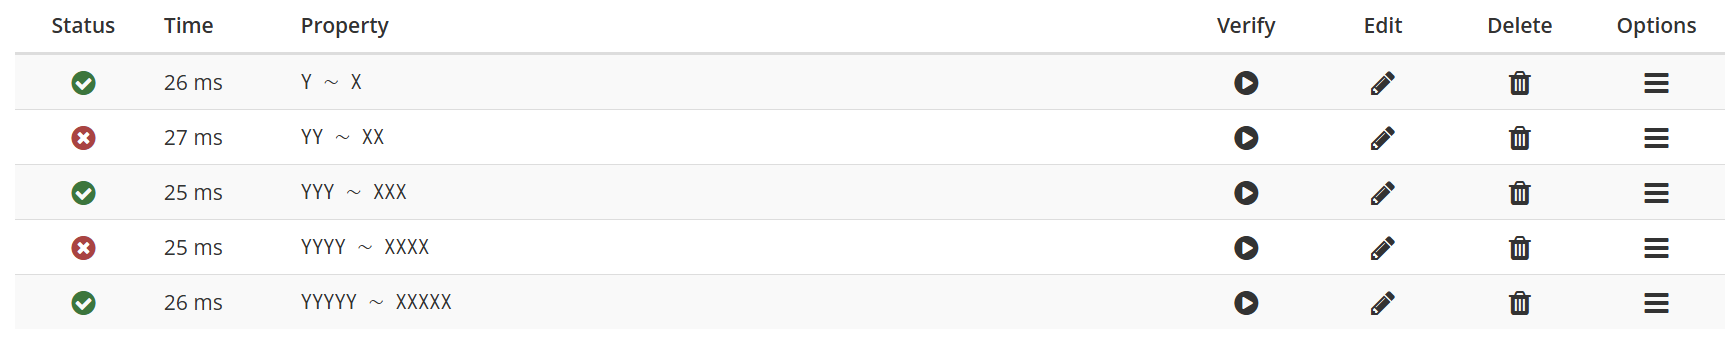
\includegraphics[width=1\textwidth]{uloha_2.png}
	\caption{Výsledky bisimulácii}
\end{figure}

\section{3.)}

Buď niečo robím zle alebo je to peklo... Po šiestich krokoch ma to prestalo baviť a už som to nerobil po krokoch. Tam vznikajú vnútorné cykly ktoré neviem ako sa majú odstraňovať... 
\\

Po použití dvoch pomocných protokolov sa nakoniec mi podarilo odstrániť všetky paralelizácie. Všetky bisimulácie priebežných výsledkov (ktoré boli nakoniec zbytočné) aj finálneho vyšli ako správne.  

\begin{figure}[!h]
	\centering
	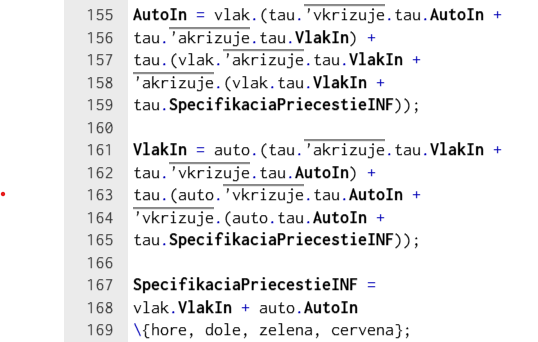
\includegraphics[width=1\textwidth]{priecestie2.png}
	\caption{Finálny výsledok}
\end{figure}


\begin{figure}[!h]
	\centering
	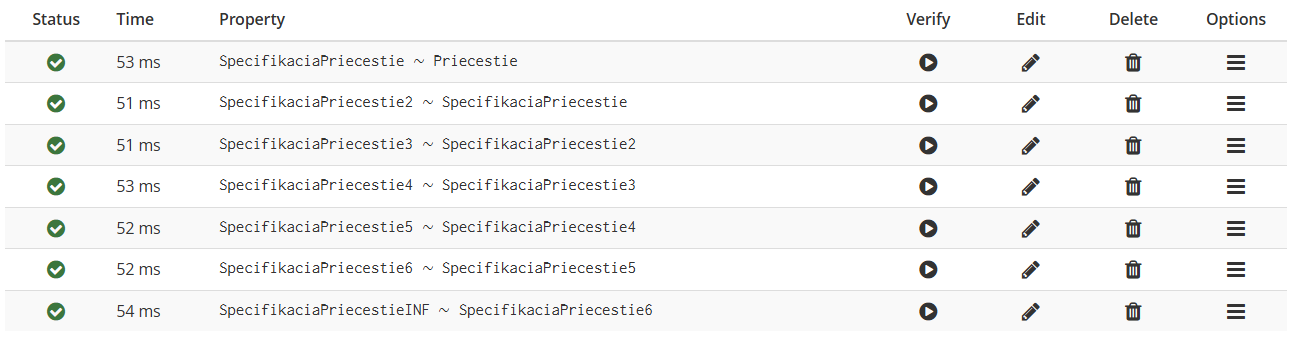
\includegraphics[width=1\textwidth]{bisim2.png}
	\caption{Výsledky bisimulácii}
\end{figure}

\end{document}